\documentclass[12pt]{article}
\usepackage[english]{babel}
\usepackage[utf8x]{inputenc}
\usepackage{amsmath}
\usepackage{graphicx}
\usepackage{caption}
\usepackage{amssymb}
\usepackage{enumitem}
\usepackage[colorinlistoftodos]{todonotes}

\begin{document}

\begin{titlepage}

\newcommand{\HRule}{\rule{\linewidth}{0.5mm}} % Defines a new command for the horizontal lines, change thickness here

\center % Center everything on the page
 
%----------------------------------------------------------------------------------------
%	HEADING SECTIONS
%----------------------------------------------------------------------------------------

\textsc{\LARGE University of California, Los Angeles}\\[1.5cm] % Name of your university/college
\textsc{\Large M152A Lab4}\\[0.5cm] % Major heading such as course name
 

%----------------------------------------------------------------------------------------
%	TITLE SECTION
%----------------------------------------------------------------------------------------

\HRule \\[0.4cm]
{ \huge \bfseries Snake}\\[0.4cm] % Title of your document
\HRule \\[1.5cm]
 
%----------------------------------------------------------------------------------------
%	AUTHOR SECTION
%----------------------------------------------------------------------------------------

\begin{minipage}{0.4\textwidth}
\begin{flushleft} \large
\emph{Group Members:}\\
Chengyu Wang\\
Simeng Pang\\
Yaowei Guo% Your name
\end{flushleft}
\end{minipage}
~
\begin{minipage}{0.4\textwidth}
\begin{flushright} \large
\emph{TA:} \\
Jia Guo % Supervisor's Name
\end{flushright}
\end{minipage}\\[4cm]

% If you don't want a supervisor, uncomment the two lines below and remove the section above
%\Large \emph{Author:}\\
%John \textsc{Smith}\\[3cm] % Your name

%----------------------------------------------------------------------------------------
%	DATE SECTION
%----------------------------------------------------------------------------------------

{\large \today}\\[2cm] % Date, change the \today to a set date if you want to be precise

%----------------------------------------------------------------------------------------
%	LOGO SECTION
%----------------------------------------------------------------------------------------

%\includegraphics{logo.png}\\[1cm] % Include a department/university logo - this will require the graphicx package
 
%----------------------------------------------------------------------------------------

\vfill % Fill the rest of the page with whitespace

\end{titlepage}

\newpage
\section*{Introduction}
We chose to implement the classical Snake game for this final project. This project requires the VGA display and the FGPA board. The players will use the buttons on the board to control the snake.\\
The rules of this game are very simple. The game map is surrounded by walls. The food will appear randomly in the map. The snake has an initial length of three. After the snake eats the food, the snake's body length will increase by 1 and the player gets 10 points. The snake has a maximum length of 16. If the snake hits the wall or collides with its own body, the snake will die. The game has three levels.
\begin{itemize}
\item After the player gets 50 points, the game enters level2 and there will be extra walls in the game map.
\item After the player get 70 points, the game enters level3. In level3, the snake moves much faster to raise game difficulty.
\end{itemize}
We use 10 modules to implement the entire design and we will explore them in the Design Section.

\section*{Design}
\subsection*{clockdiv}
This module is used to produce 5 different clocks:
\begin{itemize}
\item \textbf{segclk}: The clock for the seven-segment display.
\item \textbf{foodclk}: The clock for the eat\_food module.
\item \textbf{dclk}: The clock$(25MHz)$ for the VGA display. 
\item \textbf{sixclk}: The clock for the normal movement of the snake.
\item \textbf{fastclk}: The clock for the faster movement of the snake in level3.     
\end{itemize}
This module has the master clock signal(100MHZ) and reset as the input. We define a 25-bit register and let it increment by 1 every posedge of the master clock. We use different digits of this 25-bit register as the generated clocks.


\subsection*{gamecontrol}
This section is responsible for managing the states of the game. There are 3 modes of the game:
\begin{itemize}
\item \textbf{READY}: In this state, the snake is in the initial position of the map and has the initial body length of 3. After the players presses any button$(UP/DOWN/RIGHT/LEFT)$, the snake will start to move right.
\item \textbf{GO}: In this state, the game is going on normally. The game will remain in this state unless it receives the signal of meet\_wall or meet\_body$($which indicates that the snake hits the wall or collides with its own body$)$. Then the game will enter the DEAD state.
\item \textbf{DEAD}: In this state, the snake will flash for three times to indicate that it's dead. Then you press the reset button to restart the game. 
\end{itemize}

\subsection*{Snake\_movement}
This module is the most complicated part. A 2-dimensional array is used to record the position of each part of the snake. We can divide the work in this module into four steps:
\begin{itemize}
\item Determine the clock of the game. When the game is in level3, we need to choose the faster game clock.
\item Use the direction module to get the movement direction of the snake.
\item Determine whether the snake hits the wall or the extra walls. The mechanism is that we determine whether the snake's head is near the boundary and its direction is to the wall. For example, the snake's head is right down the wall and its direction is up, then we will assign $meet\_wl = 1$.
\item Determine whether the snake collides with its own body. The method is very easy. We simply need to judge whether the snake's head is at the same position of any part of the snake's body. To judge whether that part of the body exists$($since the body length of the snake is not fixed$)$, we need a 16-bit register. For example, if the snake has length of 4, then the register $have\_body = 16'b0000000000001111$. Here is the code snippet: \\ 
\begin{minipage}{\linewidth}
            \centering
            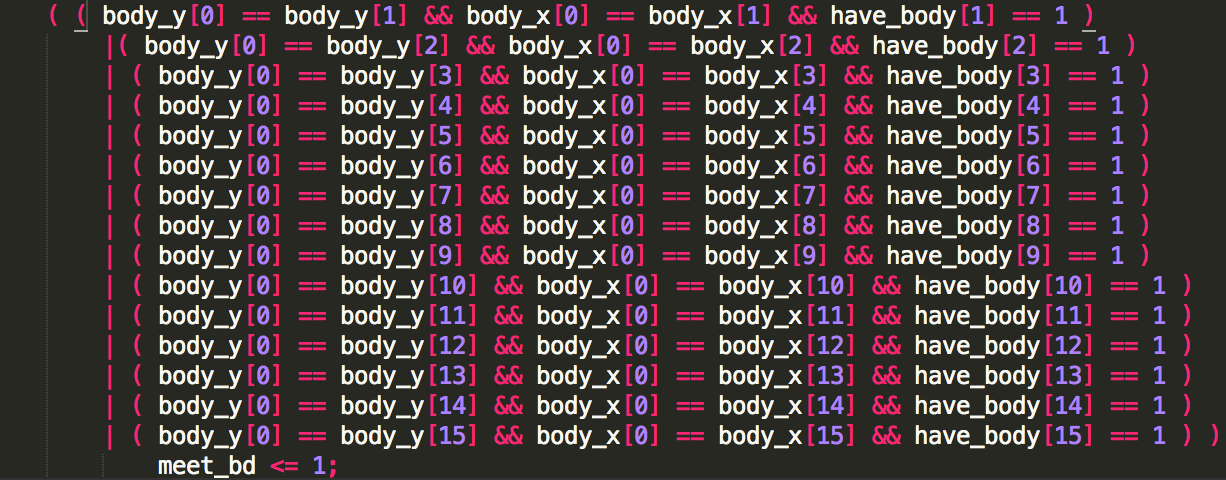
\includegraphics[width=12cm, height=5.9cm]{judgebody.png}
           % \captionof{figure}{Output Waveforms}
           % \label{fig:figure1}
        \end{minipage} 
\item Change the position of the snake. After we ensure that the snake will not be dead in this direction, we need to change the position of the snake. The snake head's position can be changed easily based on the direction. For the rest of the snake's body, we assign every part's previous connected part position to it. Here is the code snippet:
\begin{minipage}{\linewidth}
            \centering
            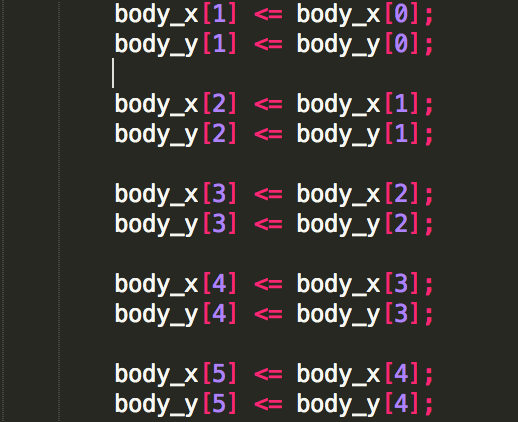
\includegraphics[width=10cm, height=5.9cm]{body.png}
           % \captionof{figure}{Output Waveforms}
           % \label{fig:figure1}
        \end{minipage} 
\item Based on the input add\_score signal, we change the body length of the snake.
\item In the $640*480$ display, each pixel is very small, so we decide to have $16*16$ pixel for each segment of the snake and wall. In this way when we check pixels, we can just check the first 6 bit of the loc\_x and loc\_y and treat the $16*16$ square as a whole. The display then becomes $40*30$. In this part inside the screen display, if the square is on the edge of the screen, signal snake is wall$(SANKE\_WALL)$, when the snake length reaches the requirement for extra wall, we set the square at our desired position to be EXTRA\_WALL, then when squares have the same positions as snake head or snake body, they are SNAKE\_HEAD or SNAKE\_BODY. Here we also have to consider the state of the snake, if the snake is in DEAD state, the snake signal should also accounts for the flash, which means the snake body is changing between SNAKE\_BODYPART and blank signal according to the dsignal. Finally we pass in the snake signal to vga\_control for display purpose.

\end{itemize} 

\subsection*{vga\_control}
This module implements the VGA display. First we set up the hsync and vsync signals as shown in nerp demo, then we define costants to represents different state snake passes in. For pixels $(x, y)$ that are inside the 640*480 display, we can decide which color to give them according to their state. For example, if the state of the pixel is snake head$(s\_start)$, we color it magenda; if the state of pixel is body$(s\_body)$, we color it green; if state is wall$(s\_wall)$, we color it yellow; if the pixel is at where the food is placed, we color it red, otherwise we leave the pixel to be black. We also have to consider the condition that when snake eats the food, the original food pixel should turn black.

\subsection*{lfsr}
This module implements the generation of random numbers. We define two registers as the x-coordinate of the food and the y-coordinate of the food. At every posedge of the master clock, the two registers are added a certain number. Since the master clock frequency is really high, the number generated will be almost random.  

\subsection*{eat\_food}
This module handles the part for generating different food positions. When the game begins or when we press the reset button, the food is placed at a fixed position. We also use random number generator to generate x and y positions for food. Then in this module, if we detect that the snake has eaten the food, we use the generated position and check whether the generated position is displayable. If the position is not in the display range, we adjust the number to be in the display range.

\subsection*{direction}
This module deals with the button input for direction for snake\_movement. Since after we press a button the snake will move to that direction constantly, we don't need a debouncer to deal with noise. We set dir and n\_dir to be right at first since the snake faces right initially. As we press a direction button, we set the certain ready\_dir to be 1, otherwise ready\_dir is 0. For each direction, it has three possible following directions$($ since the head cannot go back and overlap its own body$)$. We check if the pressed direction is feasible and set next direction to that direction. Finally we pass in the direction to snake\_movement.

\subsection*{seven\_segment}
This module takes the binary representation of the digit(4-bit register) as input and outputs the 8-digit seven segment display.



\subsection*{display\_score}
This module is used to display the score the player gains. We use four 4-bit registers to record the changes of 4 digits$($digit0 will always be 0 because the score is incremented by 10$)$. Then we adjust the anode of the seven-segment display to select which digit to be displayed. 

\subsection*{snake\_top}
This is the top module of the project. In this section we first call the $clockdiv$ module to generate different clocks. Then we call the modules $Snake\_movement, gamecontrol, eat_food, vga_control, display\_score$. Here is a diagram of the design:\\ 
\begin{minipage}{\linewidth}
            \centering
            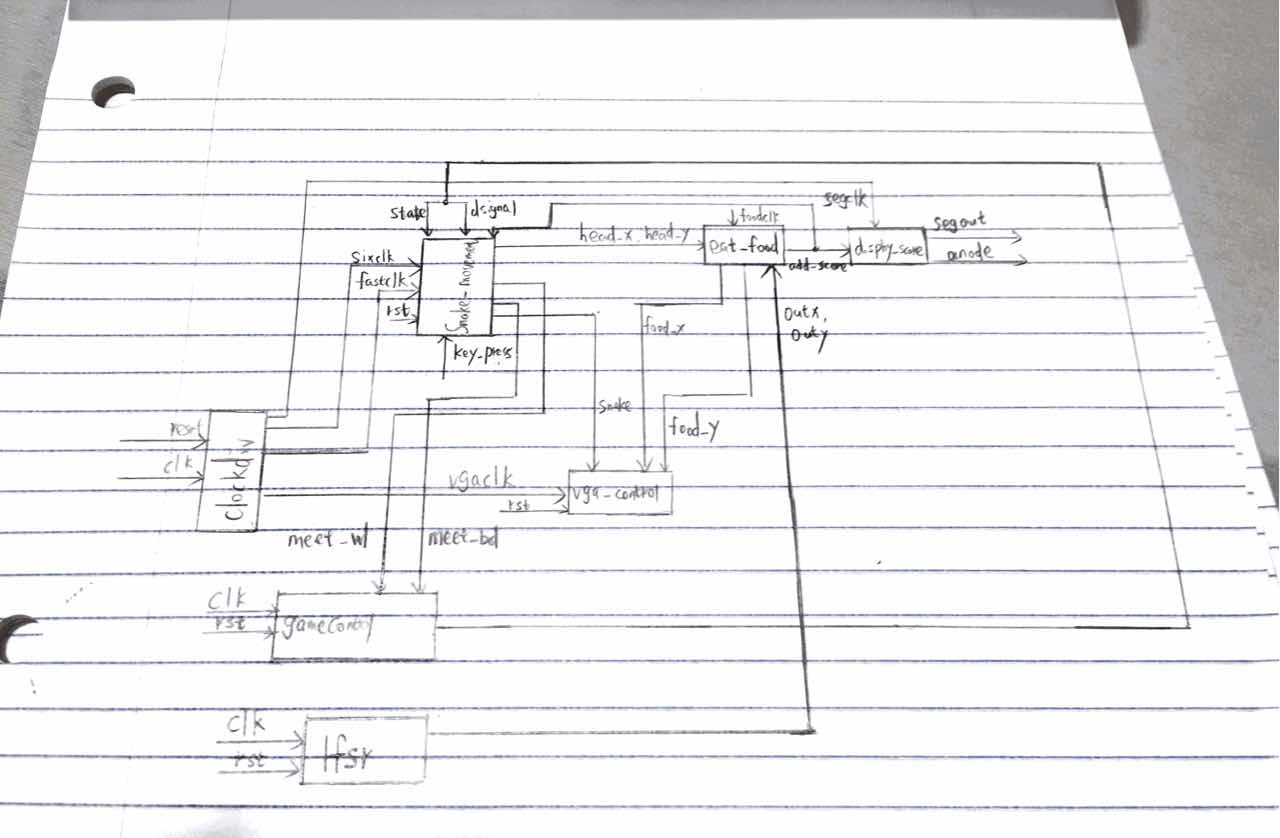
\includegraphics[width=13.8cm, height=8.4cm]{diagram.png}
            \captionof{figure}{Diagram of the Snake project}
            \label{fig:figure1}
        \end{minipage} 
        
\section*{Simulation Document}
In this part we tested our design of the snake. We tested most modules we have: clockdiv, control, direction, display\_score, lfsr, seven\_segment and vga\_control. We use both test bench and vga display to test our modules.
\\
\\
We recorded following cases: 
\begin{itemize}
\item The seven-segment display of each digit shows 0 to 9 correctly.
\\
\\
\begin{minipage}{\linewidth}
            \centering
            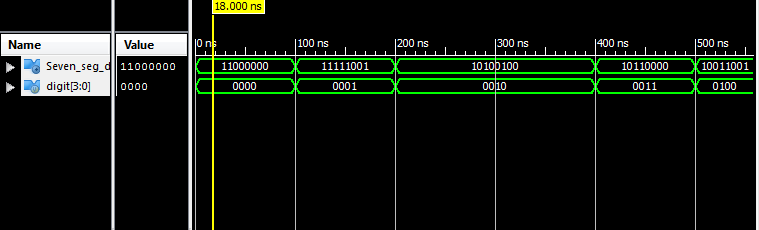
\includegraphics[width=13.5cm, height=6.2cm]{ssd.png}
            \captionof{figure}{Output of the seven-segment display. When input is a number in 0-9, it will output the certain combination of seven-segment display, when it's a number not in 0 to 9, it will output the default combination. }
            \label{fig:figure2}
        \end{minipage}
\\
\\        
\item For this project, we have a master clock, which is 100MHz. And we use this clock to create 5 new clocks. The segclk$($around 400Hz$)$ is used for ssd display, the foodclk$($around 200Hz$)$ is used to generate food, the dclk$($25MHz$)$ is used for vga display, the sixclk$($around 3Hz$)$ is the slower clock for snake movement and the fastclk$($around 6Hz$)$ is the faster clock for snake movement.
\\
\\
\begin{minipage}{\linewidth}
            \centering
            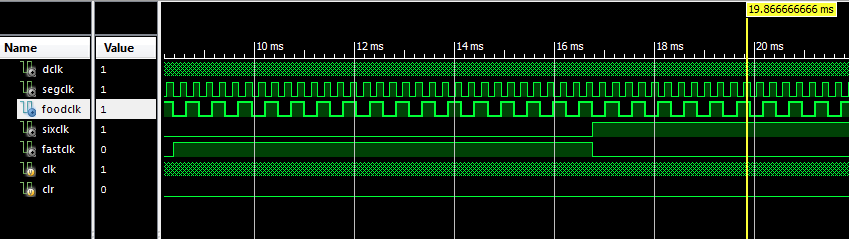
\includegraphics[width=13.5cm, height=5.2cm]{clkdiv.png}
            \captionof{figure}{Output of five clocks using clock divider. We can see that segclk is twice as fast as foodclk, fastclk is twice as fast as sixclk, and the scales are proper for all five clocks. }
            \label{fig:figure3}
        \end{minipage}
\\
\\
\item In control module, the initial state is READY, when a key is pressed it turns to GO, then when the snake hits wall or its own body, the state turns to DEAD.
\\
\\
\begin{minipage}{\linewidth}
            \centering
            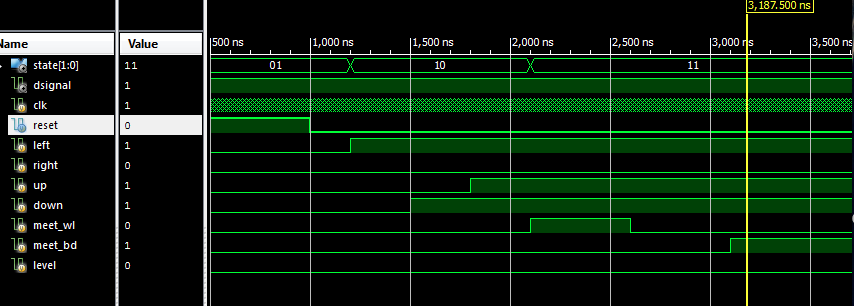
\includegraphics[width=13.5cm, height=6.2cm]{control.png}
            \captionof{figure}{Output of control module. We can see that when a direction key, left, is pressed, the state changes from 01$($READY$)$ to 10$($GO$)$ when meet\_wl changes from 0 to 1, the state changes from 10 to 11$($DEAD$)$.  }
            \label{fig:figure4}
        \end{minipage}
\\
\\
\item In the lfsr mode, we generate different positions for food each time. We also limit the range for x and y positions in order not to generate a position that is out of screen display.
\\
\\
\begin{minipage}{\linewidth}
            \centering
            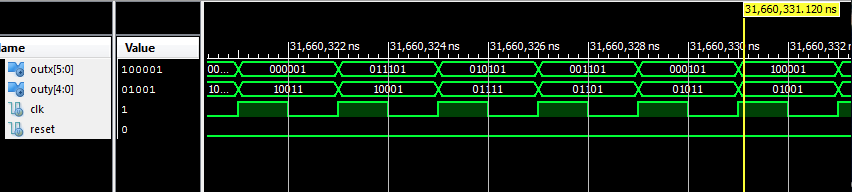
\includegraphics[width=13.5cm, height=4.2cm]{randnum.png}
            \captionof{figure}{Output of lfsr module. We can see that the values of outx and outy are different for each posedge. }
            \label{fig:figure5}
        \end{minipage}
\\
\\
\item When any direction key is pressed, the direction module outputs a corresponding direction for snake movement.
\\
\\
\begin{minipage}{\linewidth}
            \centering
            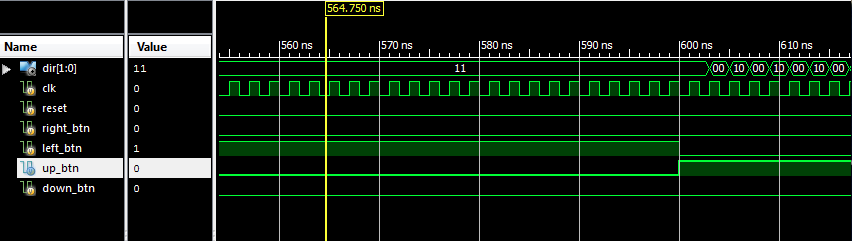
\includegraphics[width=13.5cm, height=4.2cm]{dir.png}
            \captionof{figure}{Output of direction module. When left\_btn is pressed, the dir output is 11$($right$)$, since the snake goes to right at first when any of the button is pressed, then when left\_btn is release up\_btn is pressed, the output dir changes to 10$($left$)$, when we release up\_btn, the state changes to up. }
            \label{fig:figure6}
        \end{minipage}
\\
\\
\item The snake module outputs state of the vga display, different states inside screen will have different colors in vga display, which is represented by red, green and blue signal. The color outside screen is all black.
\\
\\
\begin{minipage}{\linewidth}
            \centering
            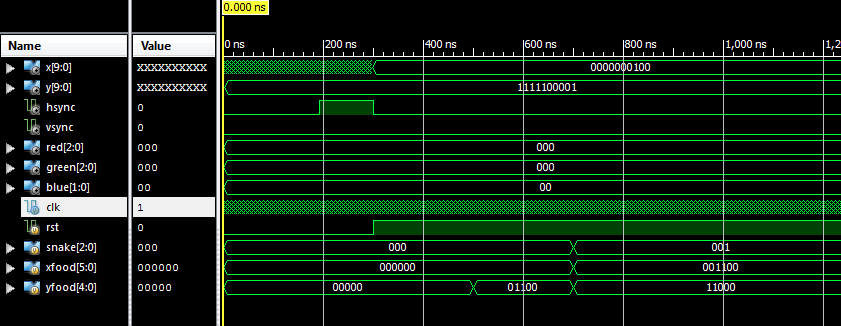
\includegraphics[width=13.5cm, height=5.2cm]{vga.png}
            \captionof{figure}{Output of vga\_control. When signal of vga is 00$($blank$)$, red, green and blue signals are all 0. When signal of vga is 01 but the position is outside screen, red, green and blue signals are also 0. }
            \label{fig:figure7}
        \end{minipage}
\\
\\
\item The snake\_movement module is the most important module in our design, it keeps snake moving, changes moving direction of snake, checks whether it goes to DEAD state, passes in display state to vga display and takes care of level of game, such as extra\_wall and speed of snake. Pressing reset sets the game back to initial state.
\\
\\
For this module, we only have 4 direction button inputs, clk input and reset input, but we have many variables changing during the process, so it's very difficult to test using test bench, and we decide to directly test on vga display.
\\
\\
\begin{minipage}{\linewidth}
            \centering
            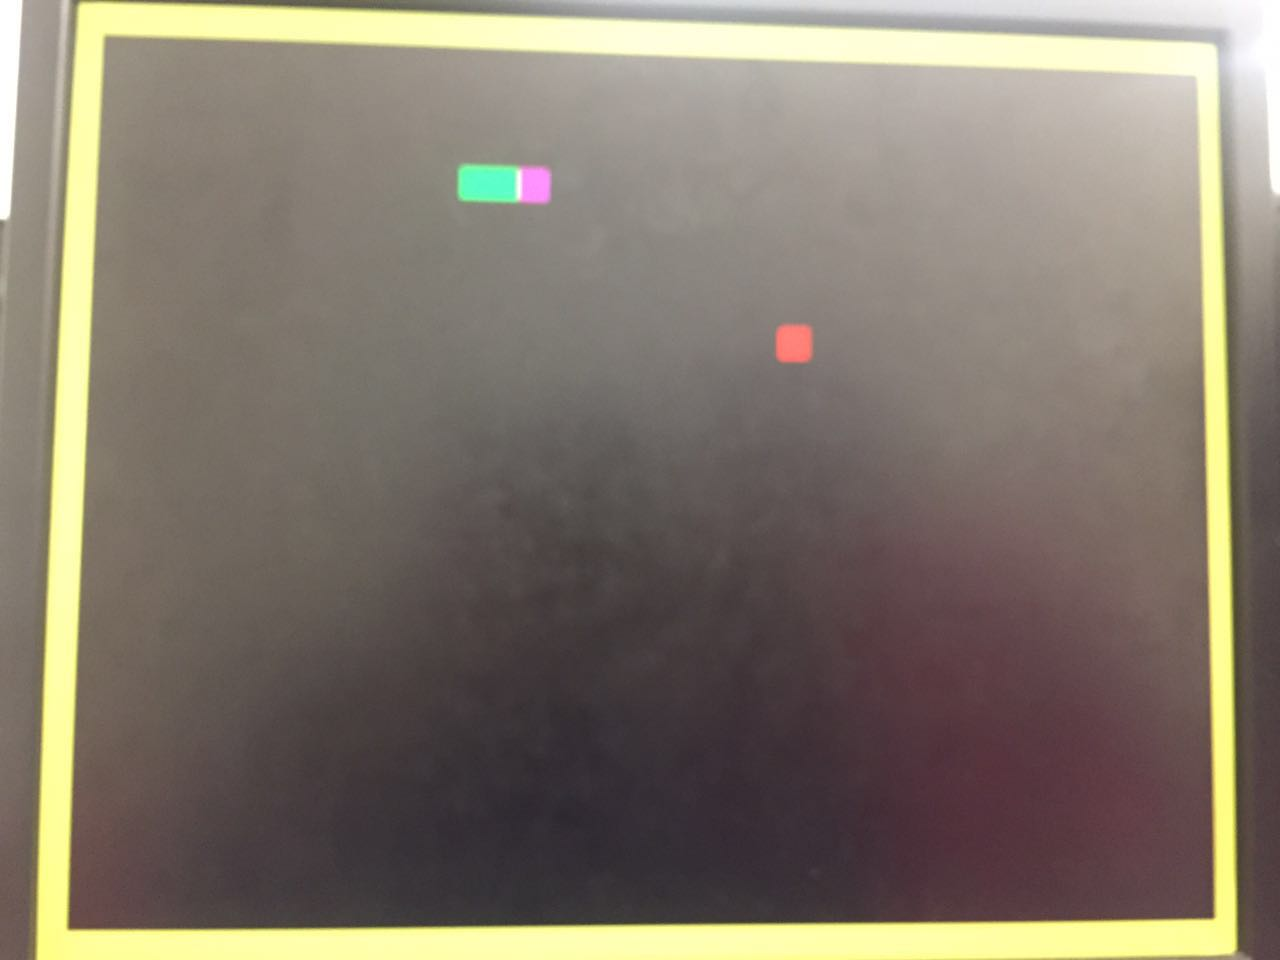
\includegraphics[width=6.5cm, height=4.5cm]{snake1.png}
            \captionof{figure}{Initial display, when we press reset, the graph also goes back this display. }
            \label{fig:figure8}
        \end{minipage}
\\
\\
When the snake eats one food, the length of the snake increses by 1. The initial length is 3, then 4, 5, 6... When the length reaches 7 and score reaches 5, the extra\_wall appears.
\\
\\
\begin{minipage}{\linewidth}
            \centering
            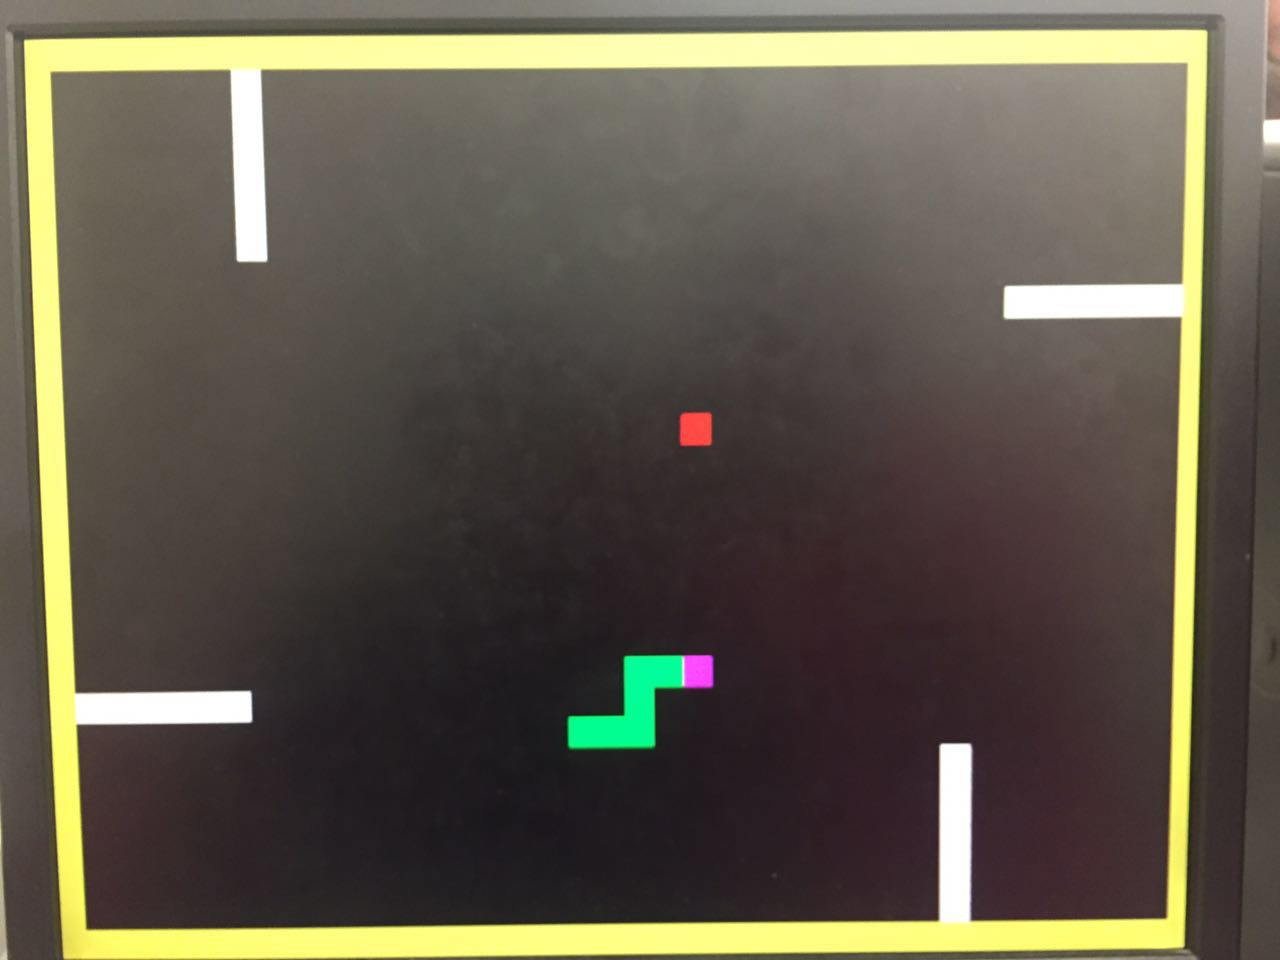
\includegraphics[width=6.5cm, height=4.5cm]{snake2.png}
            \captionof{figure}{Display with extra\_wall, at this time the length of snake is bigger than or equal to 7.}
            \label{fig:figure8}
        \end{minipage}
\\
\\
When length reaches 9, the speed of snake increases, but we cannot show in graph.
\\
\\
When snake hits wall or its own body, meet\_wl or meet\_bd becomes true, the snake is dead and flashes for three times. We let snake hit different edge of the wall, including hitting extra wall from different directions, we also let snake hit different segment of its body, they all work fine, flash for three times and stops moving after that.
\\
\\
\begin{minipage}{\linewidth}
            \centering
            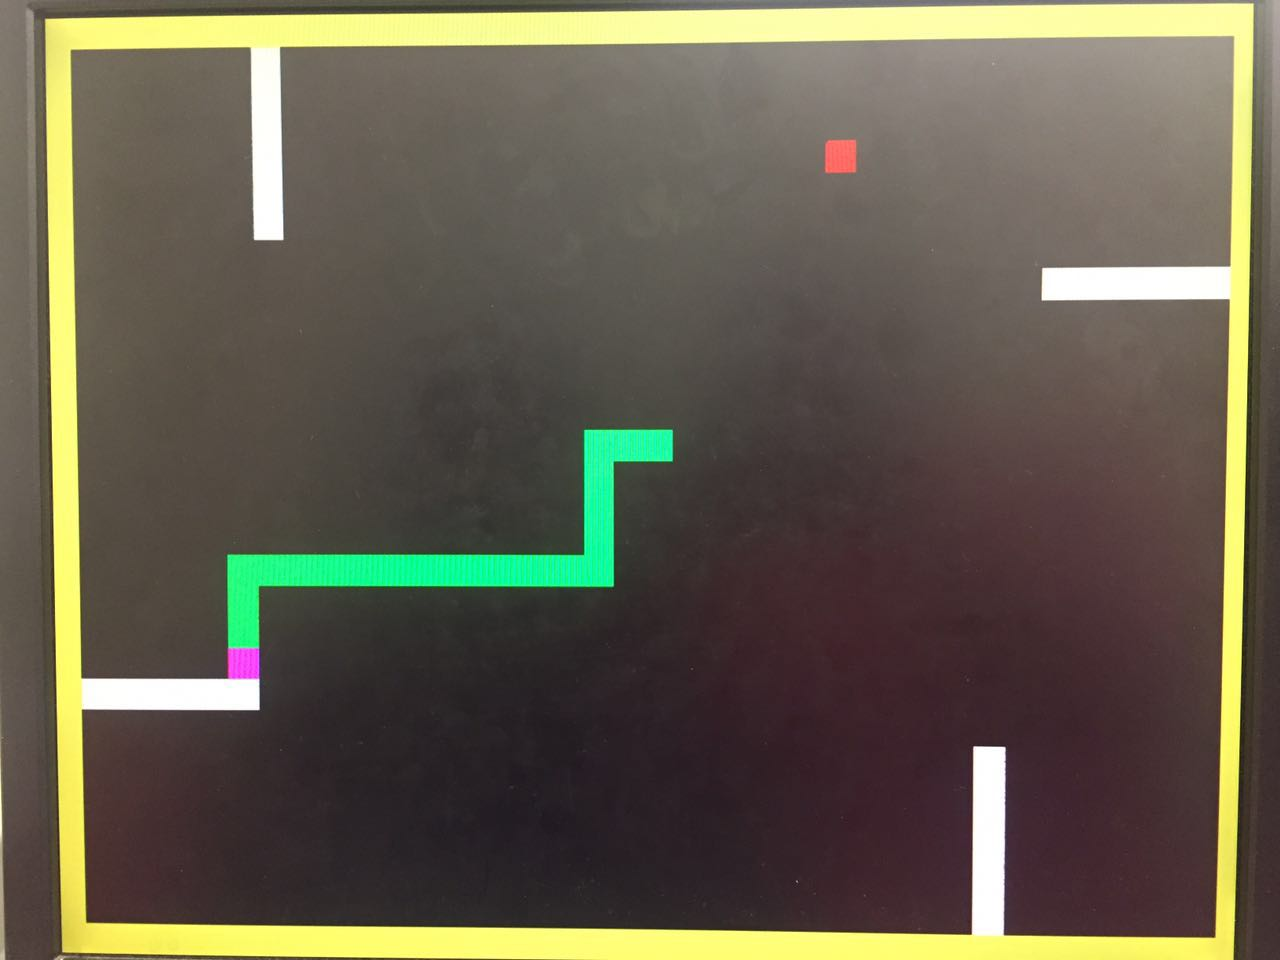
\includegraphics[width=6.5cm, height=4.5cm]{snake4.png}
            \captionof{figure}{Display about snake hitting extra wall.}
            \label{fig:figure8}
        \end{minipage}
\\
\\
 
\end{itemize}

        
\section*{Bugs}
\begin{itemize}
\item When we first played the game, the display worked fine, but as long as we pressed a button, the snake flashed for three times, which means it enters the DEAD state. Later we found out the reason is that in the control module,in PLAY state we check if inputs meet\_wl or meet\_bd is 1. If one of them is 1, the game enters DEAD state, otherwise it remains in PLAY state. We did not initialize meet\_wl and meet\_bd at first, so there might be some random nonzero numbers in it. So when control module checks these two variables, it returns that it's not zero so enters DEAD state. So we initialize these two variables to zero and the snake goes to the desired direction when we press the button.
\item When we did the extra wall section at first, we judge the position of the extra walls in the if section of judgement of normal walls$($which means we first judge whether it's the wall, and then judge whether is's the extra wall$)$. The display is not correct. Then we foundd out that the judgement of extra walls and normal walls should be in parallel but not nested. We changed the structure to if else and get the right display. 
\item We want to use the faster clock for the level3 game. However, at first when the game entered level3, the snake stopped moving and the game is like stopped. This bug took us a very long time, and then we found out that we missed a line of the clock\_div module when it is called in the top module and did not pass in the clock parameter we need. It's really weird because we thought it should be a syntax error but the compiler does not report. It works fine after we put the missing line back. 
\end{itemize}


\section*{Conclusion}
This final project gives us the opportunity to explore possible applications of FGPA board and learn about useful modules such as VGA. The biggest challenge for us is to control the pixels correctly for VGA display. It took us a long time to figure out how to control pixels in a collective way but not individually. It's also kind of difficult to connect the movement of each segment of snake body. Since this is an individual project, we had to learn many things that were not mentioned in the class, such as how to define local constants(localparam), the use of mod operator and generation of random numbers. The test of the game is somewhat hard because some features must be tested in the game display but not in the simulation, but having testbench code is still helpful. The final version of the game meets every requirement in the rubrics and adds some new features. This project really helps us better understand the Verilog language and the fundamentals of digital design. 


\end{document}